\chapter{\Large Iteración III: “Priorización de alertas”}
    El objetivo de asignar distintos niveles de prioridad a las alertas generadas por los eventos que suceden, radica en la naturaleza de estos últimos, su importancia y la gestión de la atención de los analistas del CSIRT. Esto se debe a las necesidades de optimizar el uso de los recursos técnicos y humanos del centro de respuesta a incidentes. \par

    \begin{section}{Reglas y prioridades}
    En Security Onion, la definición de los incidentes se encuentran en las reglas, que son utilizadas por los componentes IDS basados en firmas, para detectar eventos. Las reglas comprenden una serie de campos que describen con precisión la naturaleza de un incidente dado y por lo tanto, existen tantas reglas como amenazas detectadas en circulación. \par
    Las reglas tienen un conjunto de campos donde se detallan características del paquete y su contexto, tales como el puerto de origen y destino, protocolo empleado, etc y campos dedicados a la naturaleza del incidente (clasificación, mensaje, prioridad, etc). Algunos de ellos son comunes a todas las reglas y permiten agruparlas para administrar eficientemente las alertas generadas, cuando una regla coincide con la descripción de un incidente. Dado que los campos también se pueden considerar \textit{observables}, es posible utilizarlos en TheHive para gestionar incidentes y crear casos. \par
    La estructura de una regla comprende dos partes bien definidas: un encabezado (header) que es obligatorio  y un conjunto de campos opcionales. Dentro del \textit{header} encontramos la acción (alerta, notificación, etc), el protocolo (tcp, udp), puertos de origen y destino, el sentido del evento (entrante o bidireccional) y las direcciones IP de origen y destino. \par
    La segunda parte incluye dos tipos de campos: los que describen la naturaleza del evento y aquellos que contienen información del paquete de datos. Dentro del primer grupo encontramos a msg (descripción del evento), sid (id de la firma), classtype (clasificación de reglas o alertas), priority (prioridad de la firma y/o alerta), target (especifica de qué lado está el objetivo, es decir puerto de origen y puerto de destino), entre otros. El segundo grupo contiene datos extraídos que provienen de todos los niveles de la pila OSI. Se pueden mencionar a los campos “GeoIP” (localización geográfica de la IP), “Fragbits” (presencia del bit de fragmentación), “ACK” (presencia del campo ACK en paquete TCP), “itype” (número del tipo de mensaje ICMP), “http.method” (tipo de método HTTP usado), entre otros.
    \begin{figure}[H]
    \centering        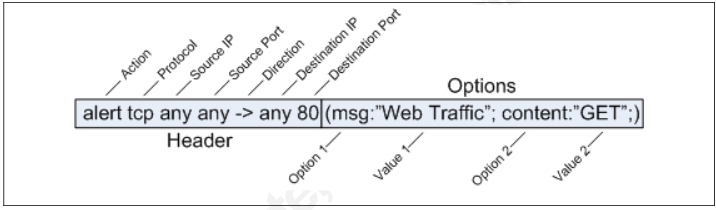
\includegraphics[width=0.7\textwidth]{./iteracion_3_imagenes/figura_41_estructura_regla.png}
    \caption{Estructura general de una regla}
    \label{fig:figura_41_estruc_regla}
    \end{figure}
    \FloatBarrier
    Como los campos están presentes en todas las reglas, es posible hacer uso de algunos de ellos para agrupar reglas que describen amenazas pertenecientes a un mismo grupo o categoría de malware: intentos de intrusión, reconocimiento, escalado de privilegios, etc y por lo tanto son útiles para gestionar los incidentes. \par
    Fue posible gestionar la configuración a través de un archivo que relaciona los siguientes campos: categorías de eventos y prioridades de la alerta generada. Este archivo llamado “\textit{classification.config}” se encuentra bajo el directorio que almacena las reglas descargadas desde diversas fuentes. En este archivo se relacionan los campos “classtype” con “priority”, de tal manera que cualquier regla cuyo campo classtype contenga a los descritos en este archivo, generará una alerta con prioridad definida también en este último. Se observa el mencionado archivo en la Figura \ref{fig:figura_43_classf_config}.
    \begin{figure}[H]
    \centering        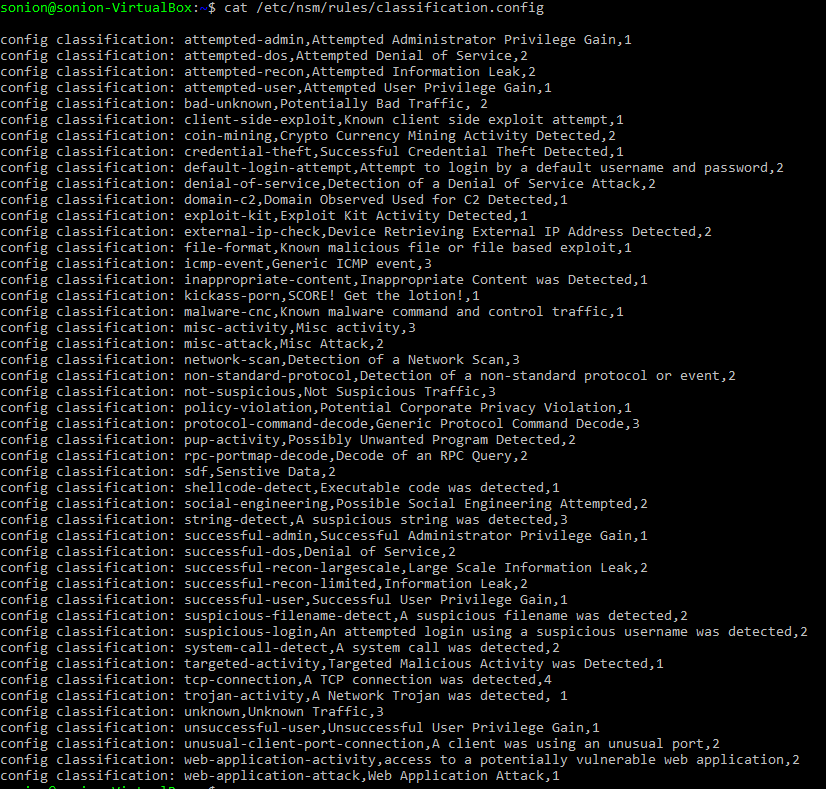
\includegraphics[width=1\textwidth]{./iteracion_3_imagenes/classification-config.png}
    \caption{Archivo \textit{classification.config}}
    \label{fig:figura_43_classf_config}
    \end{figure}
    \FloatBarrier
    Se observa en la Figura \ref{fig:figura_43_classf_config} tres campos separados por comas. El primero corresponde a la categoría del evento, el segundo a un mensaje que puede ser utilizado para la alerta y el último campo indica el nivel de prioridad. Este utiliza valores numéricos para representar el grado de importancia de los eventos pertenecientes a cada categoría, siguiendo una escala decreciente donde uno (1) representa la máxima prioridad. \par
    De esta manera, fue posible administrar un enorme número de reglas agrupadas en un reducido grupo de categorías y modificar el nivel de prioridad asociadas a ellas, esto tuvo impacto en las alertas que generaba el sistema y su visualización. \par
    \begin{subsection}{Necesidad de automatización de alertas}
    La naturaleza de los incidentes determina su elegibilidad para una respuesta automatizada al tener en cuenta por un lado su estructura bien conocida y por el otro su alta tasa de repetición en un periodo determinado. En estos casos, sería inútil destinar recursos como la atención de un analista que ya conoce perfectamente el comportamiento de este tipo de eventos y por lo tanto la respuesta apropiada a estos. También se incluyen aquellos casos en los que aún conocida su estructura, el incidente proviene en simultáneo de múltiples fuentes en muy poco tiempo, de manera que la capacidad humana de responder de a un evento a la vez resulta sobrepasada y por lo tanto, ineficiente. Estos son los casos de ataques de reconocimiento y los de denegación distribuida de servicio (DDoS), entre otros. \par
    Una de las maneras de llevar a cabo esta automatización es mediante el uso de los responders de Cortex (sección \ref{ref-cortex}) o bien mediante ElastAlert (sección \ref{seccion4-5}). Este último resulta menos conveniente que Cortex, ya que el mantenimiento a largo plazo de los \textit{scripts} necesarios es difícil debido a las diferencias entre las versiones de ElastAlert. En este proyecto se realizaron experiencias de laboratorio con Cortex, las cuales no llegaron a pasar a la fase de producción. 
    \end{subsection}

    \end{section}

    \begin{section}{Verificación de RF5: Definición de criterio para priorizar alertas.}
    
    Se dispuso de aproximadamente cuarenta y siete (47) categorías de incidentes disponibles por defecto, en este proyecto consideramos para el máximo nivel de prioridad a siete clasificaciones dado su nivel de ocurrencia y nivel de impacto para la organización. Las categorías a las que asignamos el máximo nivel de prioridad fueron las siguientes:
    \begin{itemize}
    \item \textit{Web-application-attack}: esta categoría engloba a un conjunto enorme de \textit{malware} y ataques a nivel de capa de aplicación. Gusanos, \textit{ransomware}, ataques de reconocimiento entre otras amenazas comparten esta categoría. Sobre el caso particular de los ataques de reconocimiento, se aplicaron filtros para separarlos de los demás ya mencionados.
    \item \textit{Unsuccessful User}: intentos repetidos de ganar acceso en activos e infraestructura de la organización.
    \item \textit{Attempted-dos}: intentos de ataque de denegación de servicio y su variante distribuida (DDoS).
    \item \textit{Known client side exploit attempt}: intento de ejecución de \textit{exploits} en el lado del cliente.
    \item \textit{Exploit Kit Activity Detected}: detección de actividad de un kit de \textit{exploits}.
    \item \textit{A suspicious filename was detected}: detección de nombres de archivos sospechosos.
    \item \textit{Network Trojan}: detección de un virus troyano de red.
    \end{itemize}
    
    Para verificar el cumplimiento del requerimiento funcional 5, se procedió a editar el archivo  classification.config que se encuentra en el path /etc/nsm/rules/. En la Figura \ref{fig:squert-L2} se observa la detección de un incidente de reconocimiento en Squert. Este incidente pertenece a la categoría “attempted-recon” y en el archivo \textit{classification.config} esta categoría tiene un nivel de prioridad 2, tal como se muestra en la figura (barra vertical naranja). Esto se puede observar con más detalle al analizar los campos de la alerta en Kibana, como se muestra en la Figura \ref{fig:Kibana-L2}. Se remarcó el campo “priority”, donde se vio que efectivamente el valor de la prioridad es 2.
    \begin{figure}[H]
    \centering
    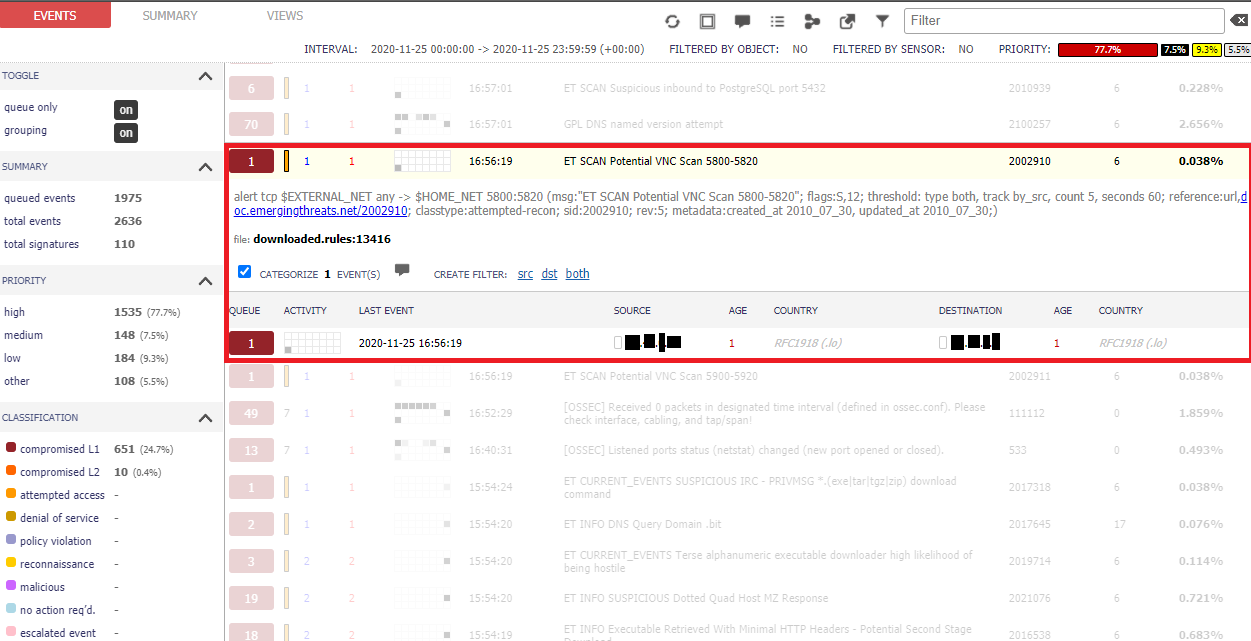
\includegraphics[width=1\textwidth]{./iteracion_3_imagenes/squert_ataque_vnc_L2-EDITADO.png}
    \caption{Incidente de reconocimiento en Squert. Prioridad nivel 2}
    \label{fig:squert-L2}
    \end{figure}
    \begin{figure}[H]
    \centering
    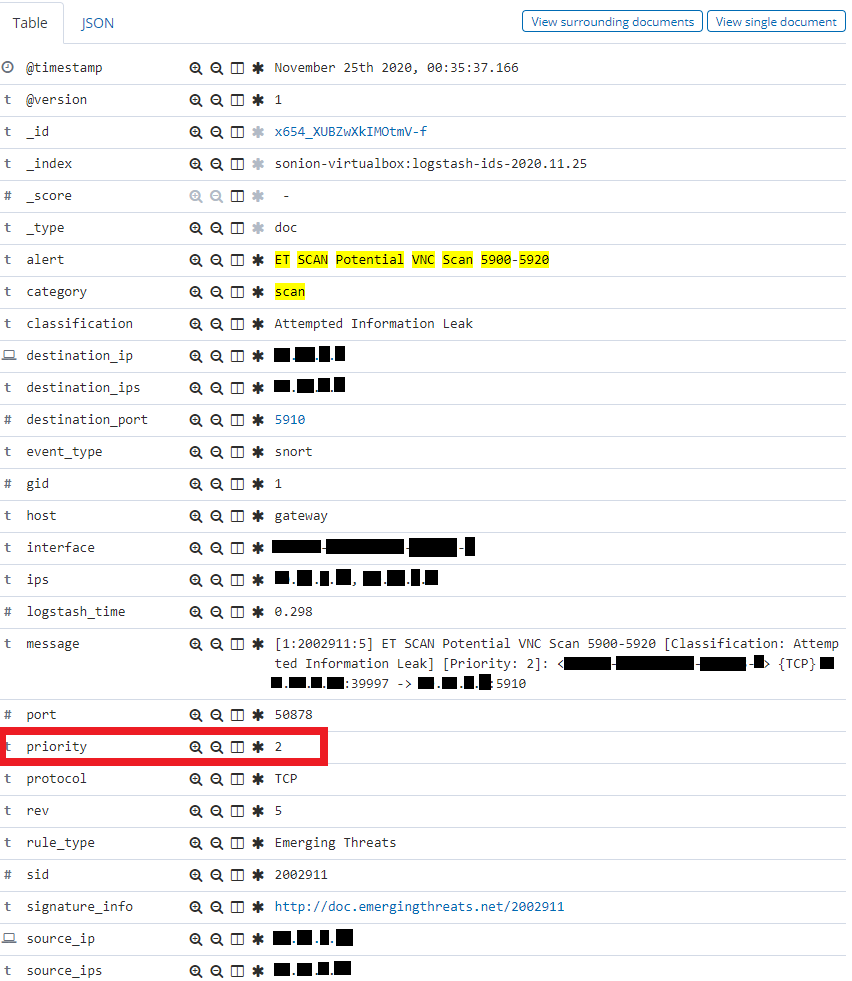
\includegraphics[width=1\textwidth]{./iteracion_3_imagenes/kibana_ataques_L2_1EDITADO.png}
    \caption{Incidente de reconocimiento en Kibana. Prioridad nivel 2}
   \label{fig:Kibana-L2}
    \end{figure}
    \FloatBarrier
    Se modificó el archivo \textbf{classification.config} para elevar el nivel de prioridad de los eventos asociados a la categoría “\textit{attempted-recon}”, que pasó del nivel 2 al nivel 1. Posteriormente se reiniciaron los sensores mediante el comando “\textit{so-sensor-restart}” y se procedió a comprobar los resultados de la modificación. Se repitió el ataque de reconocimiento y se pudo observar en las Figuras \ref{fig:squert-L1} y \ref{fig:kibana-L1} que Squert detectaba el ataque con prioridad 1 (barra vertical roja) y en Kibana se observó que el campo “priority” contenía el valor 1. Con esto se da por cumplido el requerimiento funcional 5.
    
    \begin{figure}[H]
    \centering
    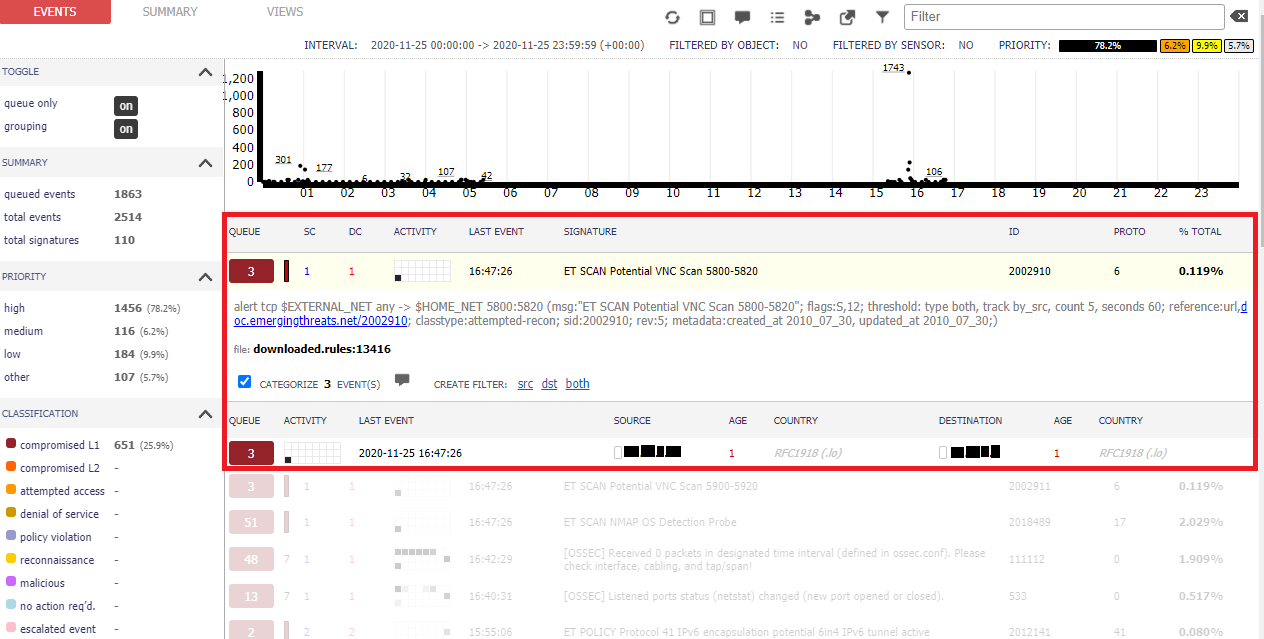
\includegraphics[width=1\textwidth]{./iteracion_3_imagenes/squert_ataque_vnc_L1-EDITADO.png}
    \caption{Incidente de reconocimiento en Squert. Nivel 1}
    \label{fig:squert-L1}
    \end{figure}
    \begin{figure}[H]
    \centering
    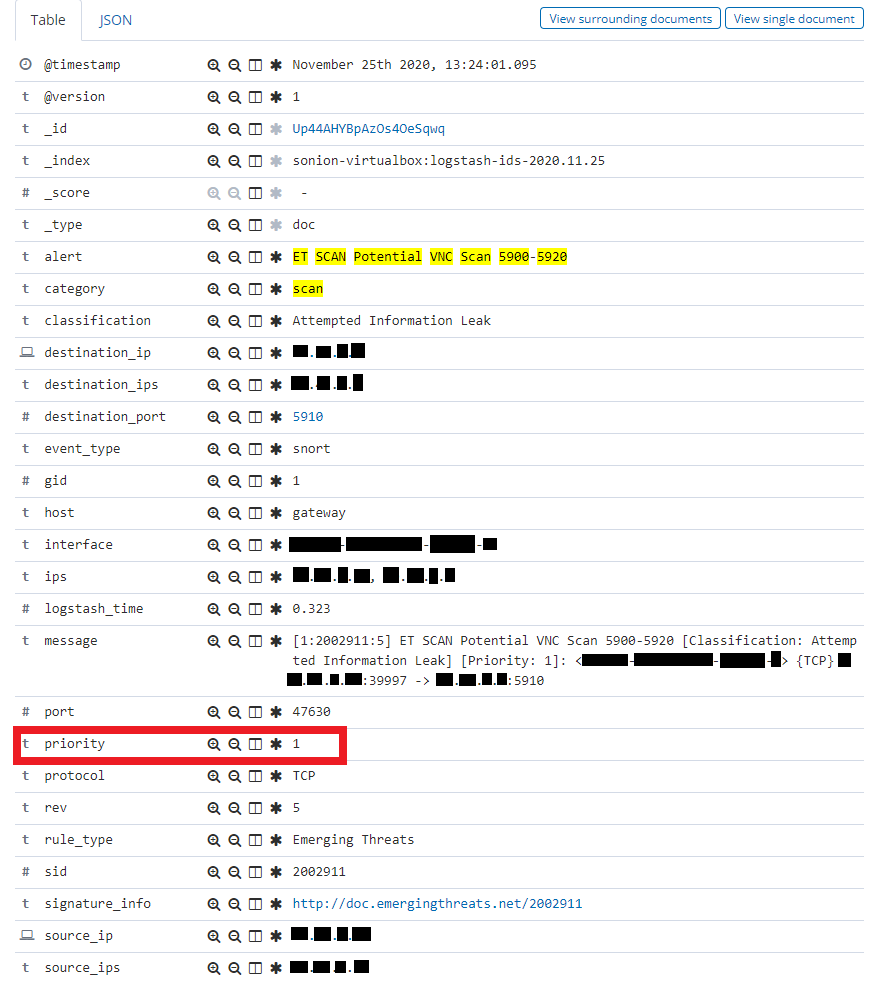
\includegraphics[width=1\textwidth]{./iteracion_3_imagenes/kibana_ataques_L2_2-EDITADO.png}
    \caption{Incidente de reconocimiento en Kibana. Nivel 1}
    \label{fig:kibana-L1}
    \end{figure}
    
    \end{section}
    \begin{section}{Pruebas de laboratorio}
    Para evaluar la capacidad del sistema de detectar distintos tipos de amenazas, se construyó un laboratorio de máquinas virtuales, simulando un escenario de aplicación real del SIEM. Para ello, se empleó el hipervisor de virtualización VMware ESXi \cite{vmware}, en el cual se desplegaron máquinas virtuales y redes según se puede observar en la Figura \ref{fig:laboratorio-sim}:
    \begin{figure}[H]
    \centering
    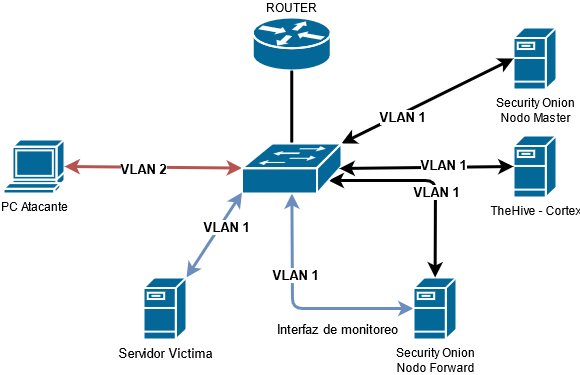
\includegraphics[width=1\textwidth]{./iteracion_3_imagenes/Propuesta_de_laboratorio_de_ataques.png}
    \caption{Diagrama topológico del laboratorio}
    \label{fig:laboratorio-sim}
    \end{figure}
    \FloatBarrier
    La figura \ref{fig:laboratorio-sim} describe el escenario de la simulación: Dos VLAN (VLAN 1 Y VLAN 2) conectadas a un switch, donde la VLAN 1 (enlaces de color negro y azul) contiene a la víctima y el SIEM, mientras que en la VLAN 2 (enlace de color rojo) se ubica el atacante. 
    En el cuadro \ref{table_14} se muestra una descripción general de las máquinas virtuales:
    \begin{table}[H]
    %\centering
    \resizebox{\textwidth}{!}{
    \begin{tabular}{|c|c|c|c|} 
    \hline
    Máquina Virtual &  Sistema Operativo  & Rol & VLAN \\
    \hline
    PC Atacante & Kali Linux v2020.4 & Atacante & VLAN 2 \\
    \hline
    Security Onion Nodo Master & Security Onion V16.04 & Procesar y almacenar alertas & VLAN 1 \\
    \hline
    Security Onion Nodo Master & Security Onion v16.04 & Analizar el tráfico en la red y notificar anomalías al nodo Master & VLAN 1 \\
    \hline
    TheHive - Cortex & Ubuntu v18.04 & Mostrar las alertas a los analistas del SIEM y accionar sobre el sistema  & VLAN 1 \\
    \hline
    Servidor Víctima & Ubuntu v18.04 & Alojar los sistemas que serán atacados  & VLAN 1 \\
    \hline %linea final de la tabla
    \end{tabular}
    }
    \caption{Descripción general de las máquinas virtuales}
    \label{table_14}
    \end{table}
   
    A continuación, se detallan las características de cada componente de la simulación:
    Redes:
    \begin{itemize}
        \item VLAN 1: es la red donde está conectado el SIEM y también donde se encuentra la víctima que será objetivo de los ataques realizados desde la VLAN 2. El SIEM está compuesto por los nodos Master y Forward de Security Onion, así como el servidor que aloja a TheHive - Cortex. La dirección de red es 172.16.52.96/27
        \item VLAN 2: es la red donde se encuentra el atacante. Su definicion es 172.16.52.64/27
    \end{itemize}
    SIEM:
        Comprende a los tres servidores encargados de la detección, procesamiento, almacenamiento, visualización y respuesta a las alertas generadas por tráfico malicioso. Sus componentes son:
        \begin{itemize}
            \item Nodo \textit{Master} de Security Onion: 
            \begin{itemize}
                \item CPU: 10 vCPU.
                \item Sistema Operativo: Security Onion v16.04.
                \item Memoria principal: 16 GB.
                \item Almacenamiento: 160 GB.
                \item Red:
                \begin{itemize}
                    \item Cantidad de interfaces de red: 1 (administración)
                    \item IP: 172.16.52.102
                    \item Máscara: 255.255.255.224
                    \item \textit{Gateway}: 172.16.52.97
                    \item conectado a VLAN 1
                \end{itemize}
            \end{itemize}
            \item Nodo \textit{Forward} de Security Onion: 
            \begin{itemize}
                \item CPU: 10 vCPU.
                \item Sistema Operativo: Security Onion v16.04.
                \item Memoria principal: 32 GB.
                \item Almacenamiento: 200 GB.
                \item Red:
                \begin{itemize}
                    \item Cantidad de interfaces de red: 2 (administración y monitoreo)
                    \item IP: 172.16.52.103 (interfaz de administración)
                    \item Máscara: 255.255.255.224
                    \item \textit{Gateway}: 172.16.52.97
                    \item conectado a VLAN 1
                \end{itemize}
            \end{itemize}
            \item TheHive - Cortex: 
            \begin{itemize}
                \item CPU: 8 vCPU.
                \item Sistema Operativo: Ubuntu v18.04.
                \item Memoria principal: 8 GB.
                \item Almacenamiento: 80 GB.
                \item Red:
                \begin{itemize}
                    \item Cantidad de interfaces de red: 1 (administración)
                    \item IP: 172.16.52.101
                    \item Máscara: 255.255.255.224
                    \item \textit{Gateway}: 172.16.52.97
                    \item conectado a VLAN 1
                \end{itemize}
            \end{itemize}
        \end{itemize}
    Servidor Víctima:
    Este servidor contiene a la aplicación web DVWA, que junto al servidor serán objeto de ataques. 
     \begin{itemize}
                \item CPU: 4 vCPU.
                \item Sistema Operativo: Ubuntu v18.04.
                \item Memoria principal: 8 GB.
                \item Almacenamiento: 100 GB.
                \item Red:
                \begin{itemize}
                    \item Cantidad de interfaces de red: 1 (administración)
                    \item IP: 172.16.52.105
                    \item Máscara: 255.255.255.224
                    \item \textit{Gateway}: 172.16.52.97
                    \item conectado a VLAN 1
                \end{itemize}
            \end{itemize}
PC Atacante:
Desde esta computadora se realizaran los ataques al servidor víctima, para ello se utilizaran herramientas y \textit{scripts} disponibles en el sistema operativo Kali Linux.
    \begin{itemize}
            \item CPU: 4 vCPU.
            \item Sistema Operativo: Kali Linux v2020.4
            \item Memoria principal: 8 GB.
            \item Almacenamiento: 100 GB.
            \item Red:
            \begin{itemize}
                    \item Cantidad de interfaces de red: 1 (administración)
                    \item IP: 172.16.52.67
                    \item Máscara: 255.255.255.224
                    \item \textit{Gateway}: 172.16.52.65
                    \item conectado a VLAN 2
            \end{itemize}
        \end{itemize}
    \begin{subsection}{Desarrollo de la experiencia de laboratorio}
    Durante esta etapa, se desarrolló un test de penetración en la red del servidor objetivo. Esto consistió en una serie de ataques contra el servidor víctima y el software que este sirve, con el objetivo de encontrar vulnerabilidades en el propio servidor así como en la aplicación web alojada y eventualmente explotar estos fallos de seguridad. La aplicación alojada por el servidor víctima fue DVWA (siglas de \textit{Damm Vulnerable Web Application}), una aplicación web diseñada para entrenamiento de técnicas de ciberseguridad en condiciones de laboratorio. Fue construida para exponer distintas vulnerabilidades que pueden ser reconocidas y explotadas, en diferentes niveles de seguridad. 
    Los ataques siguieron un esquema de fases progresivo: Reconocimiento, detección de vulnerabilidades y explotación de estas últimas.
    \begin{subsubsection}{Fase 1: Reconocimiento del objetivo}
    La meta durante esta fase consiste en recabar toda la información posible del servidor objetivo. Es la etapa más importante ya que a partir de los datos obtenidos, se observa el contexto del objetivo y las posibles vulnerabilidades que existan. La información recabada incluye el tipo de sistema operativo, puertos abiertos o filtrados, servicios web y la naturaleza de los mismos, entre otros. Un análisis detallado de estos datos permitirá avanzar en las siguientes fases del test de penetración.\par
    Existen dos tipos de reconocimiento: pasivo y activo. En el primer caso, se trata de reunir información de manera indirecta, sin entrar en contacto con el objetivo. Esto último se logra mediante la recopilación de información proveniente de fuentes abiertas, razón por la cual este tipo de reconocimiento también se conoce como OSINT (por las siglas en inglés de \textit{Open Source Intelligence}). Ejemplos de estas fuentes son resultados de buscadores, \textit{blogs}, redes sociales, servidores DNS, etc, tal como se describe en la Figura \ref{fig:osint}. Existen herramientas para automatizar y sistematizar la búsqueda de este tipo de información, como “whois” que mantiene información de registro sobre cualquier dominio web, “HTTrack” para clonar localmente sitios web, “Sublist3r” que permite encontrar todos los subdominios de una url, etc, asi como motores web que permiten rastrear múltiples fuentes de información que estén relacionadas a un dominio, IP o MAC: este es el caso de “Shodan.io”.
    \begin{figure}[H]
    \centering
    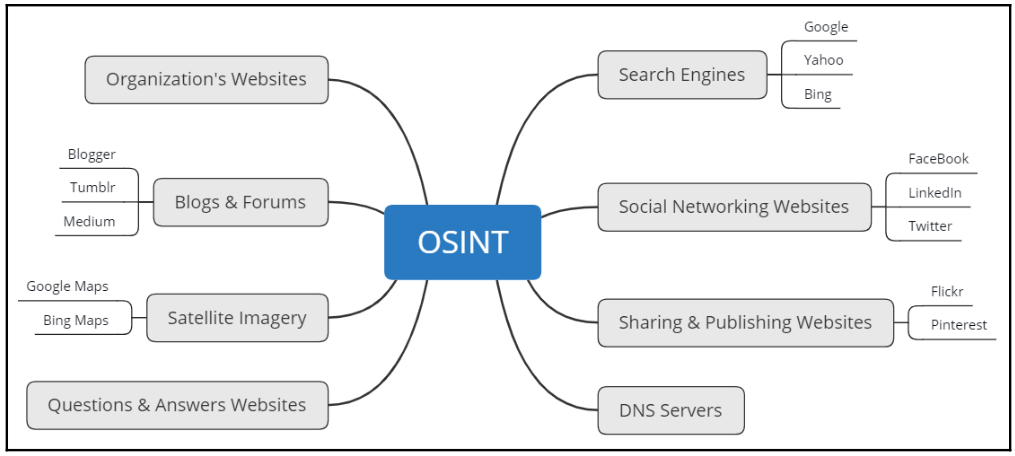
\includegraphics[width=1\textwidth]{./iteracion_3_imagenes/OSINT.png}
    \caption{Fuentes de reconocimiento indirecto (OSINT). Fuente: \textit{Kali Linux 2019 - Singh Glen}}
    \label{fig:osint}
    \end{figure}
    \FloatBarrier
    El reconocimiento activo, por otro lado, hace contacto directamente con el objetivo, de manera de recopilar información detallada que las técnicas de OSINT no pueden conseguir. El reconocimiento activo es esencial para crear un perfil detallado y preciso del objetivo, tales como el sistema operativo, puertos, los servicios disponibles y sus versiones, etc. Los resultados son usados para identificar potenciales vulnerabilidades. Este es el tipo de reconocimiento desarrollado en el laboratorio. Aunque existen muchas herramientas para llevado a cabo un ataque de reconocimiento, en esta simulación se utilizó “Nmap” y “Nessus”, junto a herramientas como “Legion”, que incluyen a Nmap, Hydra y otros \textit{scripts} para realizar ataques de fuerza bruta. Estos últimos se emplearon para realizar ataques de detección y explotación de vulnerabilidades. 
    \end{subsubsection}
    \begin{subsubsection}{Ataque de reconocimiento utilizando Nmap}
    Se utilizó Nmap \cite{nmap} para realizar ataques de reconocimiento activo ya que es posible analizar una red identificando \textit{hosts} activos, escanear puertos activos y descubrir servicios, configurando una sola línea de comandos. Por otro lado, Nmap es uno de los escáneres de red más utilizado en \textit{tests} de penetración en el mundo.\par
    El objetivo fue identificar el servidor víctima, los puertos abiertos y los servicios que estaban expuestos.
    El comando utilizado fue: 
    \begin{verbatim}
        nmap -sT -sV -O -A -T1 172.16.52.105
    \end{verbatim}
    Donde los \textit{flags} utilizados representan:
    \begin{itemize}
        \item \begin{verbatim}
        -sT    
        \end{verbatim}
         escaneo utilizando mensajes TCP SYN, ACK.
        \item \begin{verbatim}
        -sV
        \end{verbatim}
         detección de los servicios disponibles en los puertos abiertos y su información asociada.
        \item \begin{verbatim}
        -O
        \end{verbatim} 
        habilitar la detección del sistema operativo.
        \item \begin{verbatim}
        -A
        \end{verbatim}
        detección de la versión del sistema operativo
        \item \begin{verbatim}
        -T5
        \end{verbatim}
        plantilla temporizadora. La escala va desde T0 hasta T5, donde T0 permite la velocidad de escaneo más lenta y T5 la más rápida.
    \end{itemize}
    El ataque se realizó mediante la siguiente secuencia:
    \begin{enumerate}
        \item Descubrimiento del \textit{Host}: para esto, NMAP envía los siguientes paquetes:
        \begin{itemize}
            \item ICMP \textit{echo request}. Si el \textit{host} está vivo, responderá al pedido ICMP.
            \item TCP SYN al puerto 443.
            \item TCP ACK al puerto 80.
            \item ICMP \textit{timestamp request}.
        \end{itemize}
        \item Escaneo de puertos abiertos: para identificar los puertos, se analiza la respuesta a los paquetes SYN requeridos.
        \begin{itemize}
            \item Si la respuesta recibida es SYN ACK, Nmap marcará el puerto como abierto.
            \item Si la respuesta es el paquete marcado con el bit RST, Nmap considera el puerto cerrado.
            \item Si Nmap no recibe ninguna respuesta, considerará al puerto como filtrado.
        \end{itemize}
        \item Descubrimiento de servicios: cuando un puerto es marcado como abierto, Nmap escucha la comunicación de bienvenida de los servicios que usan el puerto. Esto se debe a que servicios como SSH, FTP, SMTP, etc, se anuncian a sí mismos. En el caso de no recibir un comunicado por estos puertos, Nmap envía un mensaje y compara la respuesta con una base de firmas que le permiten identificar de qué servicio se trata.
    \end{enumerate}
Se utilizo Wireshark \cite{wireshark} para capturar el tráfico de la secuencia descrita, el mismo se observa en la Figura \ref{fig:wireshark_nmap}    
 \begin{figure}[H]
    \centering
    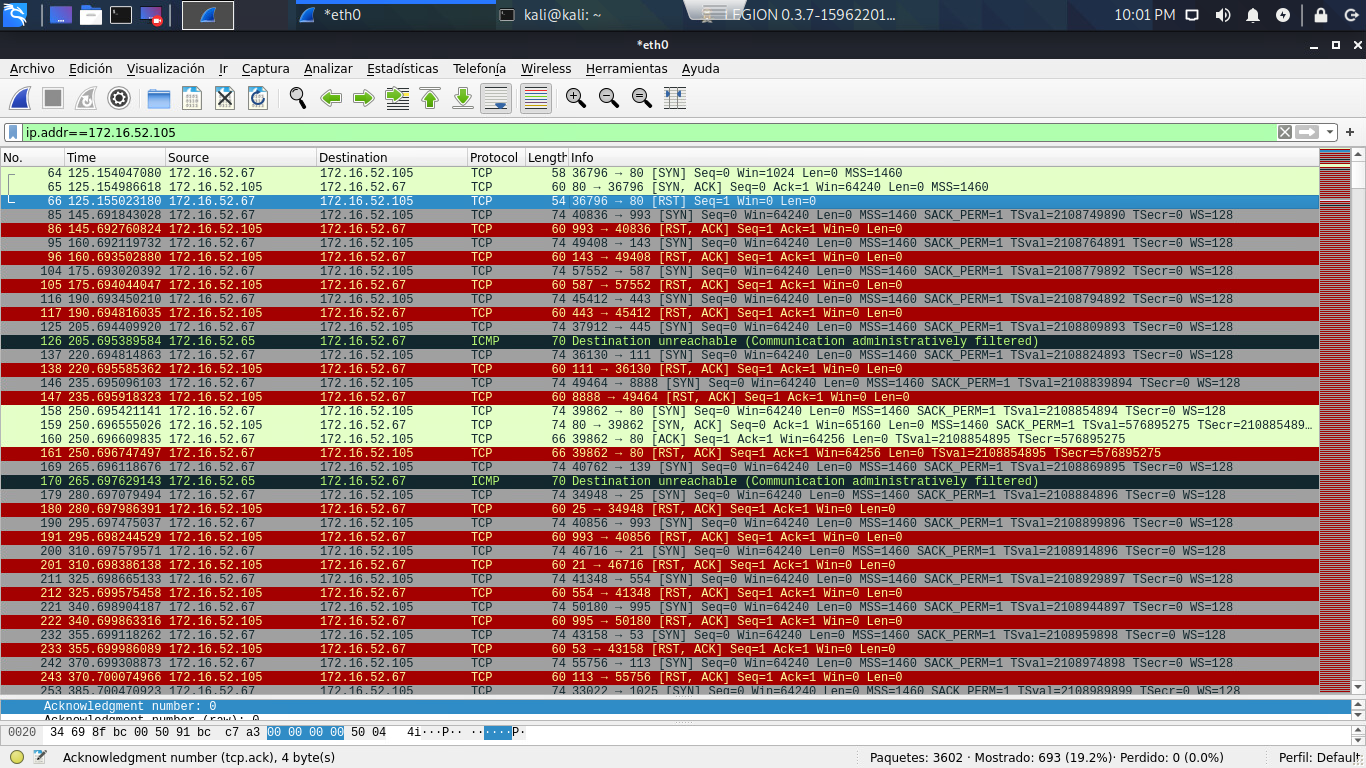
\includegraphics[width=1\textwidth]{./iteracion_3_imagenes/wireshark_NMAP.png}
    \caption{Captura del tráfico generado por NMAP al realizar el ataque de reconocimiento}
    \label{fig:wireshark_nmap}
    \end{figure}
    \FloatBarrier 
    El resultado obtenido por NMAP se observa en la Figura \ref{fig:consola_kali_nmap}
\begin{figure}[H]
    \centering
    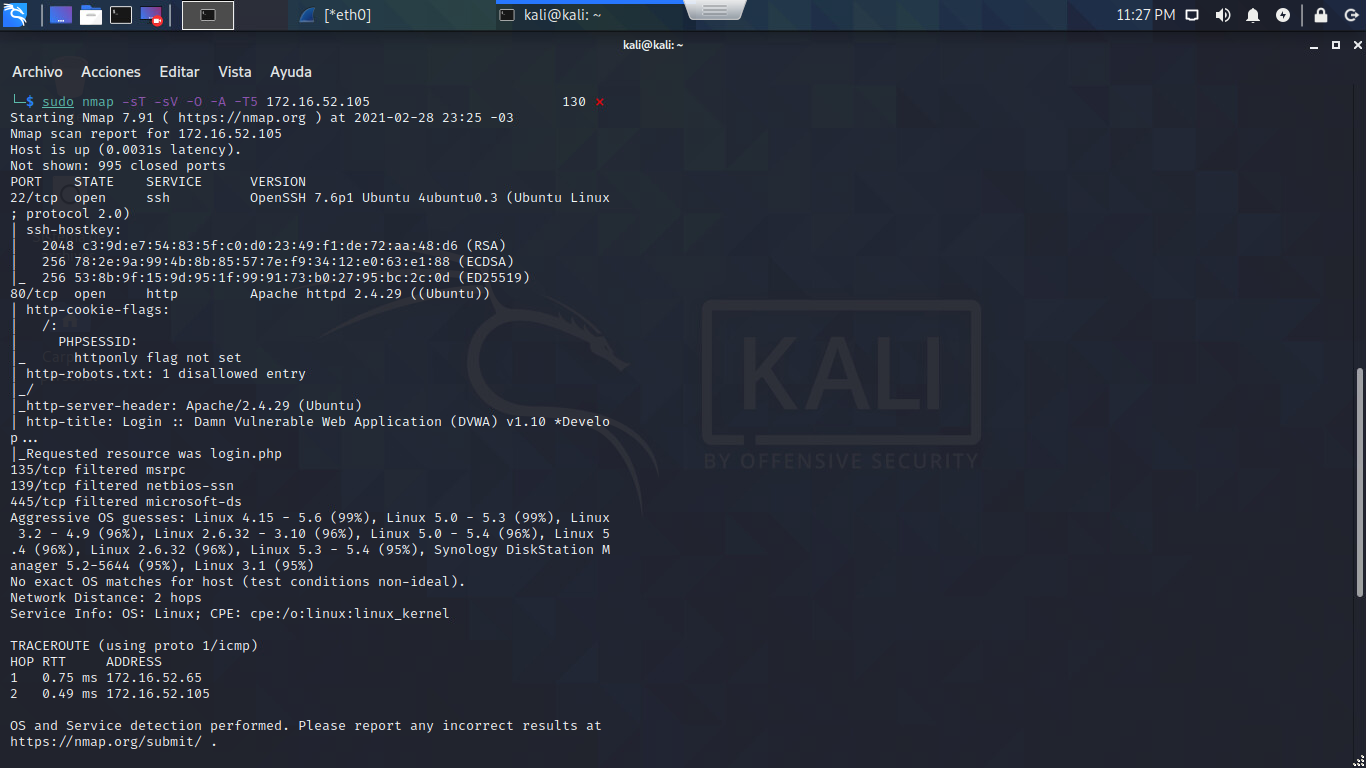
\includegraphics[width=1\textwidth]{./iteracion_3_imagenes/consola_kali_nmap.png}
    \caption{Resultados del escaneo realizado por NMAP}
    \label{fig:consola_kali_nmap}
    \end{figure}
    \FloatBarrier   
    El cuadro \ref{table_17} describe los puertos y servicios encontrados:
    \begin{table}[H]
    %\centering
    \resizebox{\textwidth}{!}{
    \begin{tabular}{|c|c|c|c|} 
    \hline
    Puerto &  Estado  & Servicio & Versión \\
    \hline
    22 & Abierto & SSH & OpenSSH v7.6p1 Ubuntu 4ubuntu \\
    \hline
    80 & Abierto & HTTP & Apache httpd 2.4.29 (ubuntu) \\
    \hline
    135 & Filtrado & - & - \\
    \hline
    139 & Filtrado & -  & - \\
    \hline
    445 & Filtrado & -  & - \\
    \hline %linea final de la tabla
    \end{tabular}
    }
    \caption{Descripción general de los puertos y servicios descubiertos}
    \label{table_17}
    \end{table}
    \FloatBarrier
    Se puede apreciar los pares de claves \textit{ssh-hostkey} en sus versiones RSA, ECDSA y ED25519. En cuanto a la aplicación, se puede observar que el \textit{flag} “httponly” de la \textit{cookie} PHPSSID no está habilitado, el \textit{header} que revela que se esta empleando apache v2.4.29 junto a un indicador de que el sistema operativo es Ubuntu. También se obtuvo el nombre de la aplicación que esta servida por la victima, mediante la captura de la variable “title” del archivo http: \textit{Damm Vulnerable Web Application}. Esto fue posible porque Nmap solicitó al \textit{webserver} el archivo “login.php”.\par
    Finalmente, si bien no hay una coincidencia exacta de la versión del sistema operativo presente en el servidor, Nmap sugiere distintas versiones de Linux  (versiones del \textit{kernel}) con altos porcentajes de probabilidad. Con esta información, es posible buscar vulnerabilidades tanto en el sistema operativo como en la aplicación web.\par
    Este ataque fue detectado por el SIEM, como se observa en la siguiente captura por parte de SQUERT, en la Figura \ref{fig:squert_nmap}.
    \begin{figure}[H]
    \centering
    \includegraphics[width=1\textwidth]{./iteracion_3_imagenes/squert-NMAP.png}
    \caption{Consola de Squert mostrando la detección del ataque de reconocimiento realizado por Nmap}
    \label{fig:squert_nmap}
    \end{figure}
    \FloatBarrier 
    En la Figura \ref{fig:thehive_nmap}, en tanto, se observa la alerta generada en TheHive: se muestra el tipo de alerta, una descripción y los campos observables. Aunque es posible agregar otros campos, los que se muestran en la  son:
    \begin{itemize}
        \item \textbf{source\_ip}: es la dirección IP desde donde se detectó al atacante. En este caso la IP del atacante es 172.16.52.67
        \item \textbf{destinatation\_ip}: es la dirección IP del objetivo atacado. En este caso, 172.16.52.105
        \item \textbf{source\_port}: es el puerto de la dirección IP desde donde se identificó el ataque. En este caso, el puerto es 59326
        \item \textbf{destination\_port}: es el puerto de la dirección IP atacada. El puerto 80 es el objetivo de este ataque.
        \item \textbf{timestamp}: marca de tiempo del momento en que se produjo la deteccion del ataque.
    \end{itemize}
    \begin{figure}[H]
    \centering
    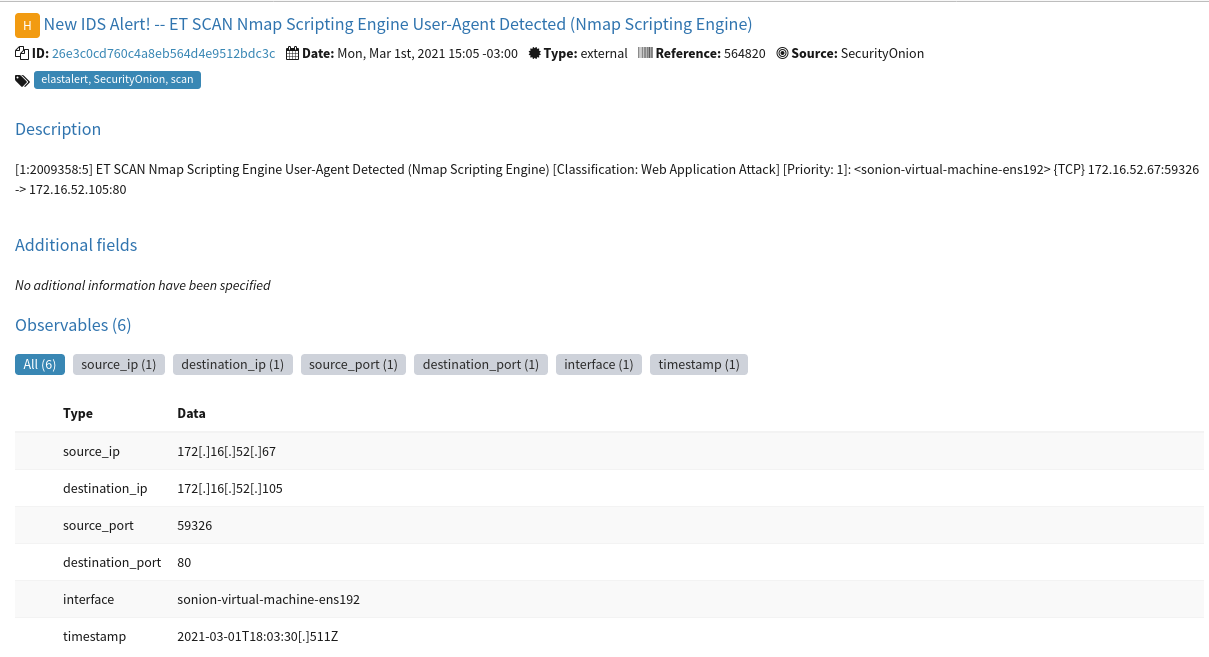
\includegraphics[width=1\textwidth]{./iteracion_3_imagenes/TheHive-NMAP.png}
    \caption{Detalle de la detección del reconocimiento, en la consola de TheHive.}
    \label{fig:thehive_nmap}
    \end{figure}
    \FloatBarrier 
    \end{subsubsection}
    \begin{subsubsection} {Fase 2: Identificación y análisis de vulnerabilidades}
    Posteriormente a la fase de reconocimiento, es necesario evaluar la información recogida para identificar potenciales vulnerabilidades en el servidor objetivo y en la aplicación web presente. \par
    Para realizar esto, se utilizó Nessus (versión \textit{Essentials})\cite{nessus}, un \textit{software} que utiliza información provista por herramientas similares a Nmap, para recabar información (o utilizar la generada por Nmap en una instancia de reconocimiento previa), para analizar los resultados y buscar en bases de datos CVE (siglas en inglés de \textit{Common Vulnerabilities and Exposures}) vulnerabilidades que puedan existir en las versiones específicas de los servicios y puertos descubiertos.\par
    En la siguientes figuras (Fig \ref{fig:nessus-1} a Fig \ref{fig:nessus-3}) se muestran los resultados, agrupados por categoría, del análisis de vulnerabilidades:
    \begin{figure}[H]
    \centering
    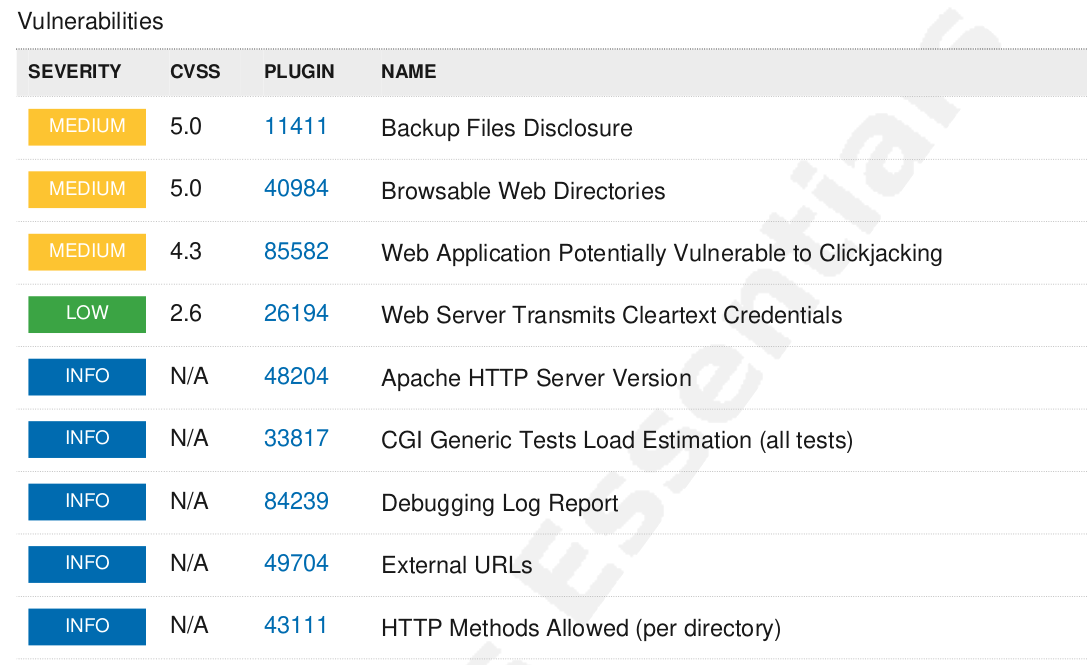
\includegraphics[width=1\textwidth]{./iteracion_3_imagenes/nessus-1.png}
    \caption{Lista de vulnerabilidades encontradas por Nessus, parte 1 de 3}
    \label{fig:nessus-1}
    \end{figure}
    \FloatBarrier 
     \begin{figure}[H]
    \centering
    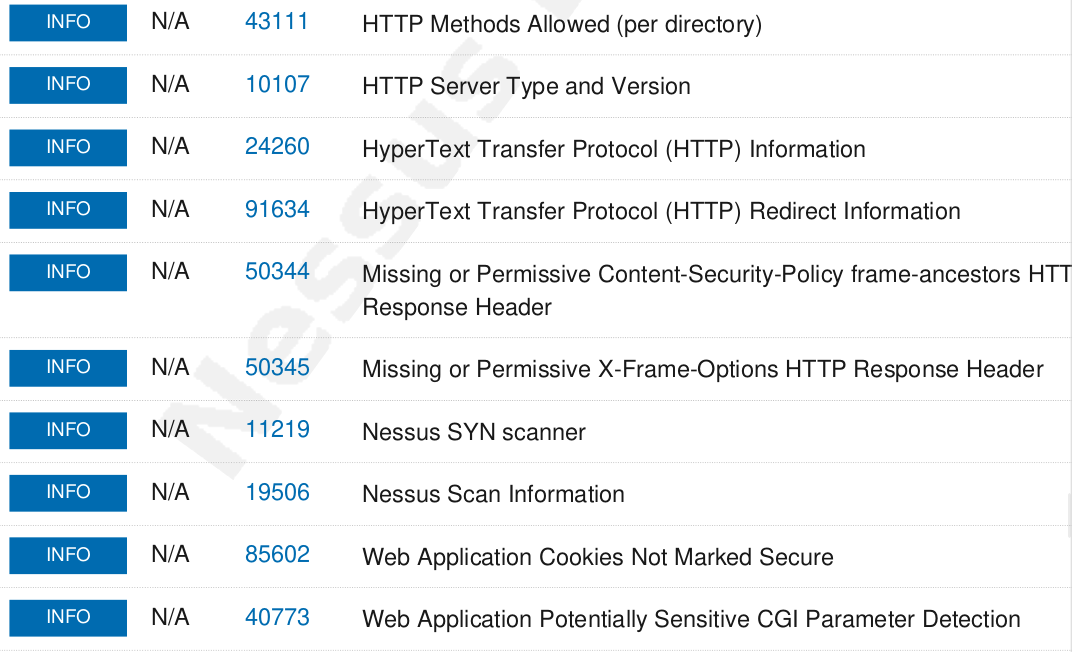
\includegraphics[width=1\textwidth]{./iteracion_3_imagenes/nessus-2.png}
    \caption{Lista de vulnerabilidades encontradas por Nessus, parte 2 de 3}
    \label{fig:nessus-2}
    \end{figure}
    \FloatBarrier 
     \begin{figure}[H]
    \centering
    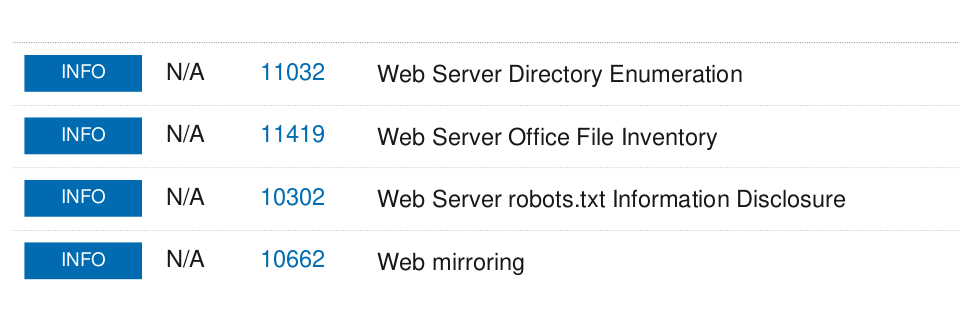
\includegraphics[width=1\textwidth]{./iteracion_3_imagenes/nessus-3.png}
    \caption{Lista de vulnerabilidades encontradas por Nessus, parte 3 de 3}
    \label{fig:nessus-3}
    \end{figure}
    \FloatBarrier 
    Se observan  exposición de archivos y directorios, métodos HTTP, información sobre las versiones de los servicios, así como vulnerabilidades particulares de la aplicación.\par
    En las siguientes figuras, se observa el detalle de algunas de las vulnerabilidades encontradas:
    \begin{itemize}
        \item Figura \ref{fig:nessus-e-1}: Divulgación de copias de seguridad. Esta vulnerabilidad permite obtener el contenido de las copias de seguridad de archivos con información sensible, agregando extensiones (.bak, .old, etc) a estos archivos. De esta manera es posible acceder a información confidencial haciendo una petición al servidor y colocando la extensión al final del archivo.
    \end{itemize}
    \begin{figure}[H]
    \centering
    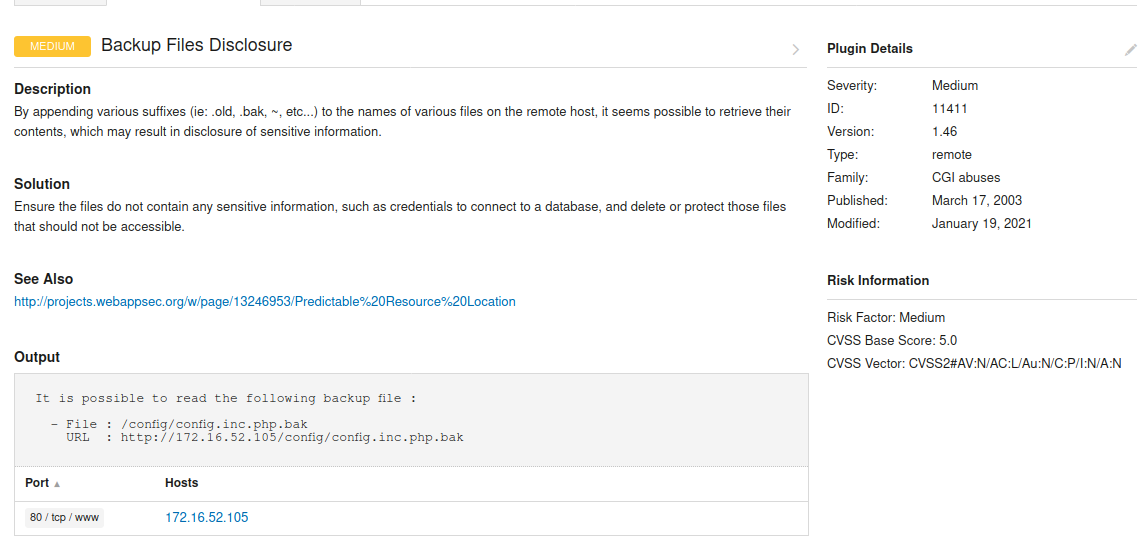
\includegraphics[width=1\textwidth]{./iteracion_3_imagenes/nessus-e-1.png}
    \caption{Divulgación de copias de seguridad}
    \label{fig:nessus-e-1}
    \end{figure}
    \FloatBarrier 
    \begin{itemize}
        \item   Figura \ref{fig:nessus-e-2}: Aplicación web potencialmente vulnerable a ataques de \textit{Clickjacking}. Esta vulnerabilidad permite a un atacante colocar \textit{iframes} (invisibles o disimulados) sobre el contenido renderizado de una página web, con el objetivo de que un usuario haga \textit{click} sobre alguno de estos elementos y de esta manera redirigirlo a una web maliciosa.
    \end{itemize}
    \begin{figure}[H]
    \centering
    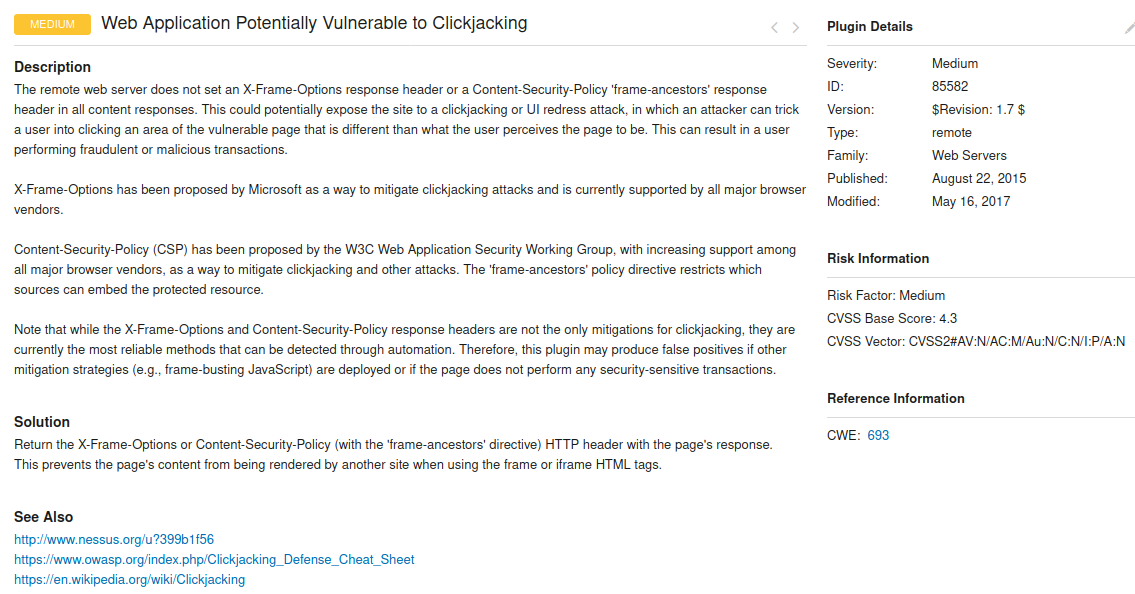
\includegraphics[width=1\textwidth]{./iteracion_3_imagenes/nessus-e-2.png}
    \caption{Aplicación web potencialmente vulnerable a Clickjacking}
    \label{fig:nessus-e-2}
    \end{figure}
    \FloatBarrier 
    \begin{itemize}
        \item  Figura \ref{fig:nessus-e-4}: Mapa del sitio web: Esta vulnerabilidad expone la estructura y contenidos con información sensible de la aplicación web, lo que permite a un atacante  elaborar acciones específicas contra esta. 
    \end{itemize}
   
    \begin{figure}[H]
    \centering
    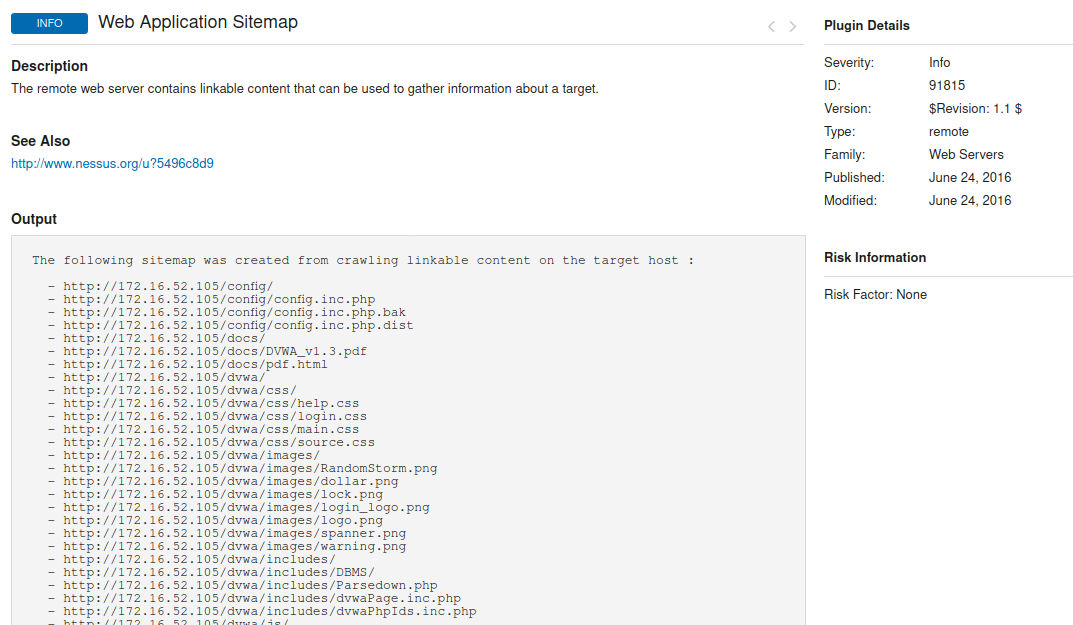
\includegraphics[width=1\textwidth]{./iteracion_3_imagenes/nessus-e-4.png}
    \caption{Mapa de sitio de la aplicacion web}
    \label{fig:nessus-e-4}
    \end{figure}
    \FloatBarrier 
    \end{subsubsection}
    \begin{subsubsection}{Fase 3: Explotación de vulnerabilidades}
    \end{subsubsection}
    \begin{subsubsection}{Ataques de inyección SQL}
    Se realizaron ataques de inyección SQL a los formularios expuestos en la aplicación web (Figura \ref{fig:sql-dvwa}), donde se utilizó el siguiente comando: \textbf{\%' and 1=0 union select null, concat(user,':',password) from users \#}
    \begin{figure}[H]
    \centering
    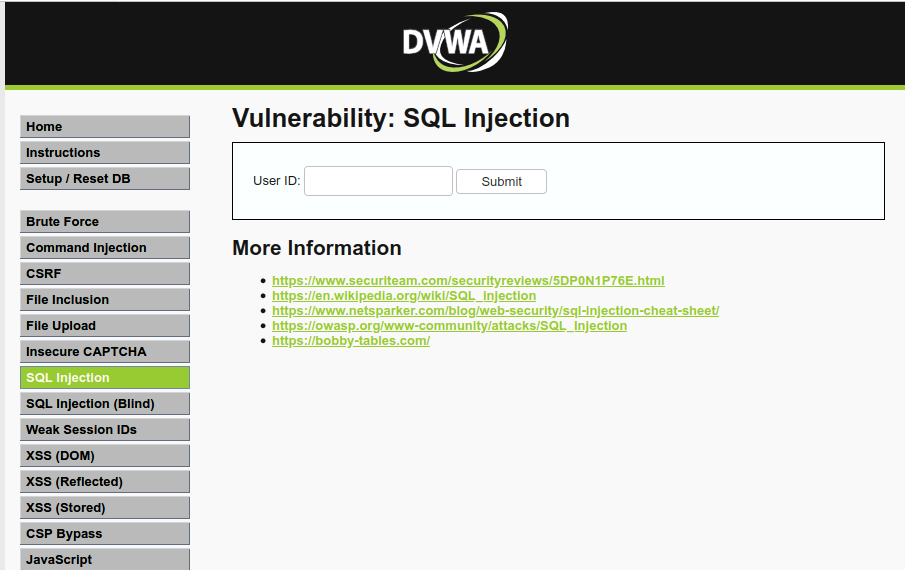
\includegraphics[width=1\textwidth]{./iteracion_3_imagenes/sql-dvwa.png}
    \caption{Formulario donde se ejecutó el comando para realizar una inyección SQL}
    \label{fig:sql-dvwa}
    \end{figure}
    \FloatBarrier 
    El ataque fue detectado por el nodo Forward de Security Onion y visible a los analistas a traves de Squert (Figura \ref{fig:sql-squert}) y TheHive (Figura \ref{fig:sql-thehive}):
     \begin{figure}[H]
    \centering
    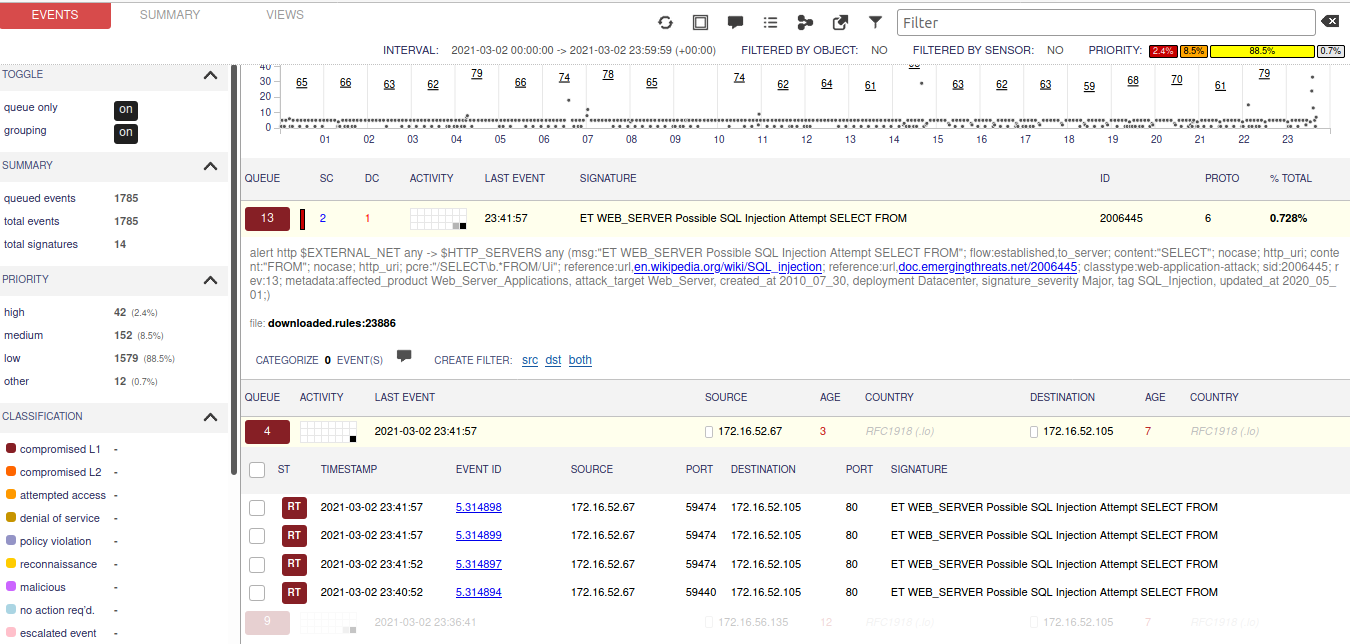
\includegraphics[width=1\textwidth]{./iteracion_3_imagenes/sql-squert.png}
    \caption{Detección del ataque de inyección SQL, observada en la consola de Squert.}
    \label{fig:sql-squert}
    \end{figure}
    \FloatBarrier 
    Luego de haber detectado el evento, ElastAlert envió la alerta correspondiente a TheHive, como se muestra en la Figura \ref{fig:sql-thehive}
    \begin{figure}[H]
    \centering
    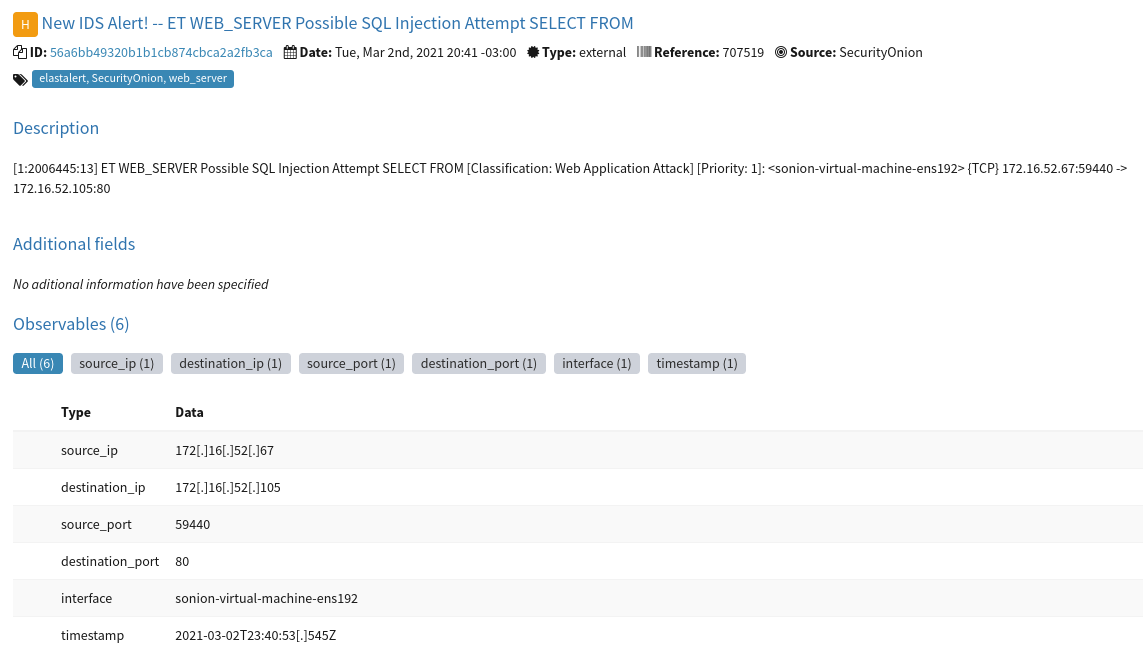
\includegraphics[width=1\textwidth]{./iteracion_3_imagenes/sql-thehive.png}
    \caption{Ataque de Inyección SQL presentado en TheHive}
    \label{fig:sql-thehive}
    \end{figure}
    \FloatBarrier  
    \end{subsubsection}
    \begin{subsubsection} {Ataques de Cross-site Scripting (XSS)}
    Se realizaron ataques de ejecución de comandos de sitio cruzado (XSS: cross-site scripting) en la aplicación DVWA. Se utilizaron scripts de Nessus destinados a probar la vulnerabilidad de una aplicación web a este tipo de ataques, probando ataques XSS almacenados y reflejados.
    Estas acciones fueron detectadas por el nodo Forward de Security Onion, como se muestra en las siguientes figuras. 
    En la Figura \ref{fig:xss-squert} se observa la deteccion de los eventos en la consola de Squert:
   \begin{figure}[H]
    \centering
    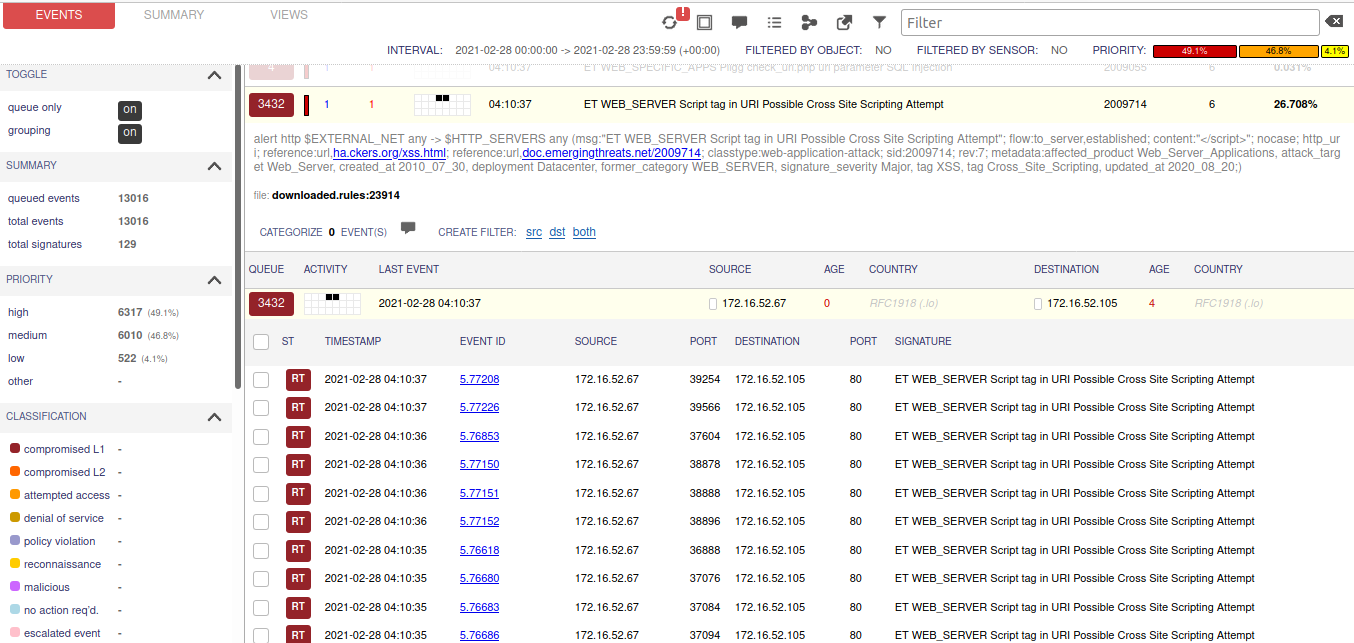
\includegraphics[width=1\textwidth]{./iteracion_3_imagenes/xss-squert.png}
    \caption{Detección de los ataques de Cross-site scripting en la consola de Squert}
    \label{fig:xss-squert}
    \end{figure}
    \FloatBarrier 
    En la Figura \ref{fig:xss-thehive} se observa la alerta generada en TheHive por ElastAlert:
    \begin{figure}[H]
    \centering
    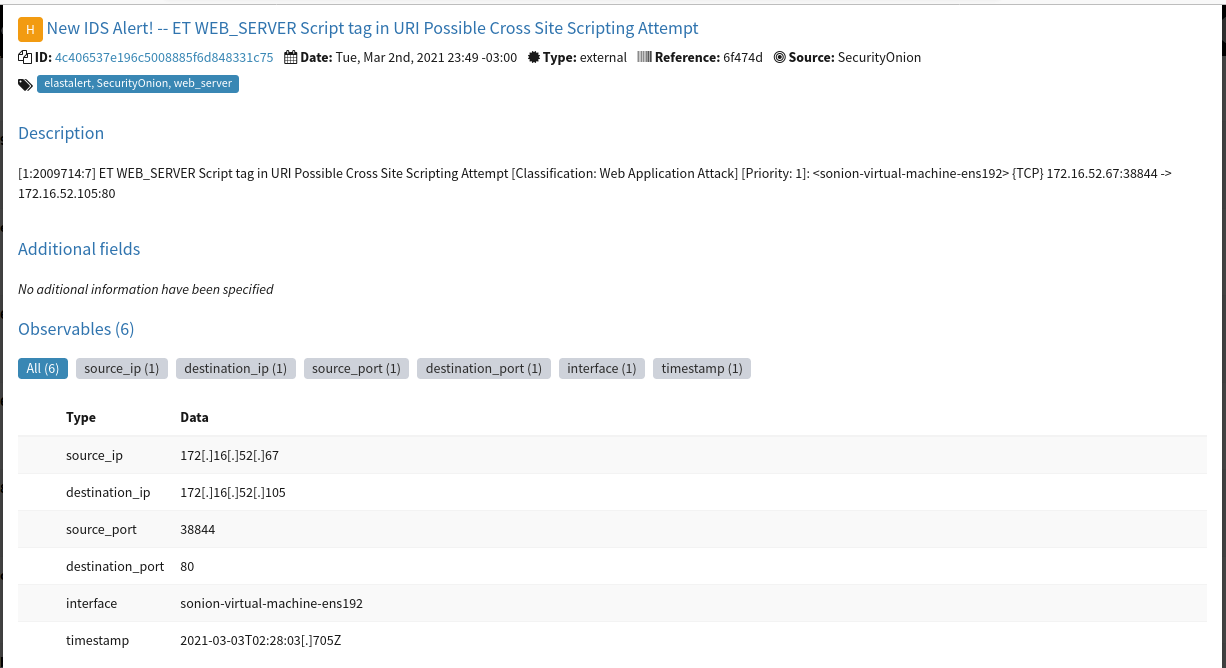
\includegraphics[width=1\textwidth]{./iteracion_3_imagenes/xss-thehive.png}
    \caption{Alerta de un ataque Cross-site Scripting presentado en TheHive}
    \label{fig:xss-thehive}
    \end{figure}
    \FloatBarrier 
    \end{subsubsection}
    \end{subsection}
    \end{section}

    \begin{section}{Corolario}
    Dado que existen incidentes que se repiten constantemente y sus comportamientos son bien conocidos por los analistas, fue necesario evitar que estos abrumaran o distrajeran la atención de los analistas. Este efecto, que se conoce como “fatiga del analista”, consiste en la pérdida de atención de los incidentes relevantes por parte del analista, ya que este los pierde de vista entre una gran cantidad de notificaciones de incidentes sin relevancia o ya conocidos. Esta situación provoca una pérdida de efectividad del SIEM y por consiguiente del CSIRT.\par
    La solución a esta situación consistió en otorgar una baja prioridad a las alertas que generaban eventos considerados de poca importancia para la organización. Luego se adaptó el sistema de notificaciones para evitar que estas abrumen a los analistas y responsables de los activos de información. 
    En cuanto a las alertas que generaban eventos considerados de baja prioridad por definición, pero que la organización considero relevantes, se aumentó su prioridad. \par
    Mediante pruebas de laboratorio, se demostró que el sistema puede detectar distintos tipos de amenazas y priorizar las que se consideran más relevantes.
    Finalmente, se consideró la futura automatización de respuestas a estos incidentes en los casos viables. \par
    \end{section}
    
